\chapter{Planung}
Es wurde zunächst ein Netzplan erstellt (Abb. \vref{fig:netzplan}), der der besseren Übersicht und Darstellbarkeit halber ab dem ersten Router nach \texttt{fire\-wall.office.axxeo.de} stark vereinfacht und auf einen weiteren Hop beschränkt ist. In der Realität folgen nach \texttt{Router eins} und \texttt{Router zwei} noch weitere Hops.
Für alle Netze außerhalb von \texttt{firewall.office.{$_{\hookleftarrow}$}\\axxeo.de} wurden private Netzbereiche gewählt, um nicht mit bereits vergebenen, öffentlichen \gls{IP}-Adressen in Berührung zu kommen.

\input{Inhalt/Grafiken/netzplan}

\section{Ressourcenplanung}
Für die Umsetzung des Projekts sind keine Anschaffungen oder speziellen Einplanungen nötig; die vorhandene Firewall \texttt{firewall.office.axxeo.de} (Abb. \vref{fig:netzplan}) wird erweitert und für Simulationen steht eine gemeinsam genutzte VMWare-Workstation bereit. Zur Erarbeitung wird ein bereits zugewiesener Standard-PC-Arbeitsplatz verwendet.

\section{Split-Access-Routing}
Um als ersten Schritt ein überhaupt laufendes Setup mit \gls{sar} zu erzeugen, wurde der im LARTC beschriebene Aufbau übernommen und den Umständen angepasst:

\begin{enumerate}
 \item Erstellen von einer \gls{Routing}-Tabelle für jedes externe Interface:\\
    \texttt{echo -e {\tq}200 one{\bs}n 201 two{\tq} {\gt}{\gt} /etc/iproute2/rt\_table}
 \item Hinzufügen von zwei Regeln in die \gls{Routing}-\gls{Policy}-Datenbank, um Antworten auf Anfragen aus den jeweils anliegenden Netzbereichen (10.1.0.0/24 und 10.2.0.0/24) auch wieder auf dem passenden Interface zu versenden:\\
    \texttt{ip rule add from 10.1.0.0/24 table one\\ip rule add from 10.2.0.0/24 table two}
 \item Hinzufügen von Routen in die im ersten Schritt erstellten Tabellen; ohne diese Einträge würden die im zweiten Schritt aufgegriffenen Pakete die jeweilige Routing-Tabelle durchlaufen, auf keinen Eintrag passen und dann wieder die main-Tabelle passieren:\\
    \texttt{ip r r 127.0.0.0/8 dev lo table one\\ip r r 10.2.0.0/24 dev eth2 src 10.2.0.1 table one\\ip r r default dev eth1 table one\\
	ip r r 127.0.0.0/8 dev lo table one\\ip r r 10.1.0.0/24 dev eth1 src 10.1.0.1 table two\\ip r r default dev eth2 table two}
 \item Ersetzen der default-Route mit einem eins-zu-eins-Balancing:\\
    \texttt{ip r r default scope global nexthop via 10.1.0.2{$_{\hookleftarrow}$}\\ {$^{\hookrightarrow}$}dev eth1 weight 1 nexthop via 10.2.0.2 dev eth2 weight 1}
\end{enumerate}

\section{Priorisierung}
Zum Verständnis von Priorisierung und Traffic-Shaping generell wurde wieder das LARTC \citep{LARTC} genutzt. Nach der Lektüre des Kapitels 9 war ersichtlich, wie die Priorisierung funktioniert und, dass die Syntax von \gls{tc} selbst weder leicht zu verstehen, noch leicht zu schreiben ist. Nach weiterer Recherche\footnote{{\ua}\url{http://tldp.org/HOWTO/HOWTO-INDEX/networking.html}} wurde ein Howto für das Tool \gls{tcng} \citep{TCNGHTB} gefunden.
Auch hier wurde nah am Beispiel gearbeitet und die Konfiguration nur wenig verändert. Die \gls{tcng}-Scripte für die Schnittstellen eth1 und eth2 auf \texttt{firewall.office.axxeo.de} sind unter \vref{lst:eth1_tcc} und \vref{lst:eth2_tcc} Angehängt.

Die Einteilung der Bandbreite für jedes Interface hat sich dabei folgendermaßen ergeben:
An eth1 steht die \gls{SDSL}-Leitung mit 2000/2000~{\kibi\bit\per\second} (Zeile \vref{lst:eth1.tcc.eth1-speed}) zur Verfügung, über welche Fernwartung via SSH erfolgen muss, da nur die auf diesem Interface liegende IP auf den Maschinen der Kunden freigeschaltet ist. An eth2 steht eine \gls{VDSL2+}-Leitung mit 50000/10000~{\kibi\bit\per\second} (Zeile \vref{lst:eth2.tcc.eth2-speed}) zur Verfügung, welche von einem weiteren Mieter im Hause betrieben wird und auf Fair-Use-Basis genutzt werden kann.

Der Aufbau der \gls{tcng}-Scripte ist hierarchisch und recht einfach; erklärt wird folgend der Aufbau des Scripts für eth1.

Als erstes wird das Interface definiert (Zeile \vref{lst:eth1.tcc.eth1}), für das \gls{tc}-Regeln erstellt werden sollen, danach wird die \gls{egress}- oder \gls{ingress}-\gls{qdisc} gewählt (Zeile \ref{lst:eth1.tcc.egress}), in der wiederum Definitionen für Traffic-Gruppen (Zeile \ref{lst:eth1.tcc.interactive-out}, \ref{lst:eth1.tcc.interactive-in}, \ref{lst:eth1.tcc.other}) und die darauf angewendeten Regeln definiert werden (Zeile \ref{lst:eth1.tcc.interactive-out-rate}, \ref{lst:eth1.tcc.interactive-in-rate}, \ref{lst:eth1.tcc.other-rate}). Verwendet wird allerdings nur die \gls{egress}-\gls{qdisc}, da nur die Datenströme wirklich beeinflusst werden können, die von der Maschine selber ausgehen.
Für alle Datenströme, die möglichst ohne Verzögerung übertragen werden sollen, sind die Klassen \emph{\$interactive\_*}  vorgesehen (Zeile \ref{lst:eth1.tcc.interactive-out-rate}, \ref{lst:eth1.tcc.interactive-in-rate}). % Ob diese Liste an Kriterien im Echtbetrieb auch wirklich den Traffic erfasst, den man hoch priorisieren will, muss noch überprüft werden\todo{umschreiben}.
Alle anderen Datenströme werden über die Klasse \emph{\$other} (Zeile \ref{lst:eth1.tcc.other}) abgewickelt.

Alle Regeln sind innerhalb des \gls{HTB} (Zeile \ref{lst:eth1.tcc.htb}) definiert. Mit der Wahl des \gls{HTB} wird versucht, einen einfachen, durchschaubaren\footnote{"`As said before, CBQ is the most complex qdisc available, the most hyped, the least understood, and probably the trickiest one to get right"' \citep[Kapitel 9.5.4.]{LARTC}} Einstieg zu finden, der laut Entwickler auch genau zum Anwendungsfall passt\footnote{"`One requirement for link-sharing is to share bandwidth on a link between multiple organizations, where each organization wants to receive a guaranteed share of the link bandwidth during  congestion, but where bandwidth that is not being used by one  organization should be available to other organizations sharing  the link."' \citep[Kapitel 2.8]{DSERV}}.
Generell erlaubt der hierarchische Aufbau eine feingranulare Aufteilung der Bandbreite nach vielen Parametern.

Für ein besseres Verständnis ist der implementierte Aufbau unter Abb. \vref{abb:tcc-tree-eth1} auch als Grafik zu sehen.

\section*{Detail-Analyse der tcng-Scripte (Listing \vref{lst:eth1_tcc} und \vref{lst:eth2_tcc})}
Die folgenden Ausführungen wurde zu einem gewissen Teil von docum.org \citep{DOCUMHTB} übersetzt, da die Formulierungen sehr treffend sind.
\begin{description}
  \item[rate] die garantierte Bandbreite einer Klasse
  \item[ceil] die maximale Bandbreite, die eine Klasse nutzen kann
\end{description}

Den Parametern \emph{rate}/\emph{burst} und \emph{ceil}/\emph{cburst} werden {\sog}\emph{\gls{token} \glspl{bucket}} zugewiesen. Der \emph{rate-bucket} wird mit \gls{token} und der \emph{ceil-bucket} mit \emph{c}\gls{token} gefüllt - es gibt also für jede Klasse zwei \glspl{bucket}. Die Geschwindigkeit mit der die Tolken gefüllt werden wird über burst und cburst festgelegt.


Ein Beispiel mit \emph{rate}=100~{\byte\per\second}, \emph{burst}=300~{\byte} und einem Datenversand von 200~{\byte\per\second}:
\begin{figure}[htb]
  \centering
  \includegraphics[height=5.5cm]{Inhalt/Grafiken/bandbreite-gewuenscht.png}
  % null.png: 1030x633 pixel, 120dpi, 21.80x13.40 cm, bb=0 0 618 380
  \caption{gewünschte Bandbreite}
  \label{fig:bandbreite-gewuenscht}
\end{figure}

\begin{figure}[htb]
  \centering
  \includegraphics[height=5.5cm]{Inhalt/Grafiken/bandbreite-nach-htb.png}
  % null.png: 1030x633 pixel, 120dpi, 21.80x13.40 cm, bb=0 0 618 380
  \caption{Bandbreite nach HTB}
  \label{fig:bandbreite-nach-htb}
\end{figure}

\begin{itemize}
  \item\textbf{0 - 3~Sekunden:} Datenversand kann in voller Geschwindigkeit erfolgen, es werden nachlaufende token und token aus dem bucket genutzt
  \item\textbf{4 - \dots~Sekunden:} bucket ist leer, es werden nachlaufende token genutzt
\end{itemize}


%Der rate-Wert bedeutet nun, dass der Rate-Bucket mit 100 token{\per\second} gefüllt wird bis er voll ist (100 token, burst). Alle weiteren token für diesen bucket werden an den ceil-bucket weitergegeben bis dieser auch gefüllt ist (300 ctoken, cburst).
%Sobald auch dieser bucket gefüllt ist, werden die token verworfen.

%Jeder token repräsentiert ein Byte - wenn also 100 Byte versandt werden sollen, werden 100 token benötigt. Beide Token werden gleich stark belastet.

%\input{Inhalt/Grafiken/token-detail}

%Es wird davon ausgegangen, dass alle Buckets gefüllt sind, da die Leitung davor nicht genutzt wurde.
%\begin{itemize}
%  \item\textbf{0 - 3~Sekunden:} der \emph{rate}-\gls{bucket} wird mit 100~token{\per\second} gefüllt und der \emph{ceil}-\gls{bucket} ist 300 ctoken groß.\\Es werden insgesamt 200~token{\per\second} genutzt, also können die überschüssigen 100~token{\per\second} in den ersten drei Sekunden aus dem \emph{ceil}-\gls{bucket} genommen werden.
%  \item\textbf{3 - \dots~Sekunden:} der \emph{ceil}-\gls{bucket} ist erschöpft und wird erst wieder aufgefüllt, wenn der \emph{rate}-\gls{bucket} mit weniger als 100~token{\per\second} belastet wird.\\Weitere Extra-token können von Eltern-Klassen, soweit vorhanden, genommen werden.
%\end{itemize}


\pgfdeclarelayer{background}
\pgfdeclarelayer{foreground}
\pgfsetlayers{background,main,foreground}
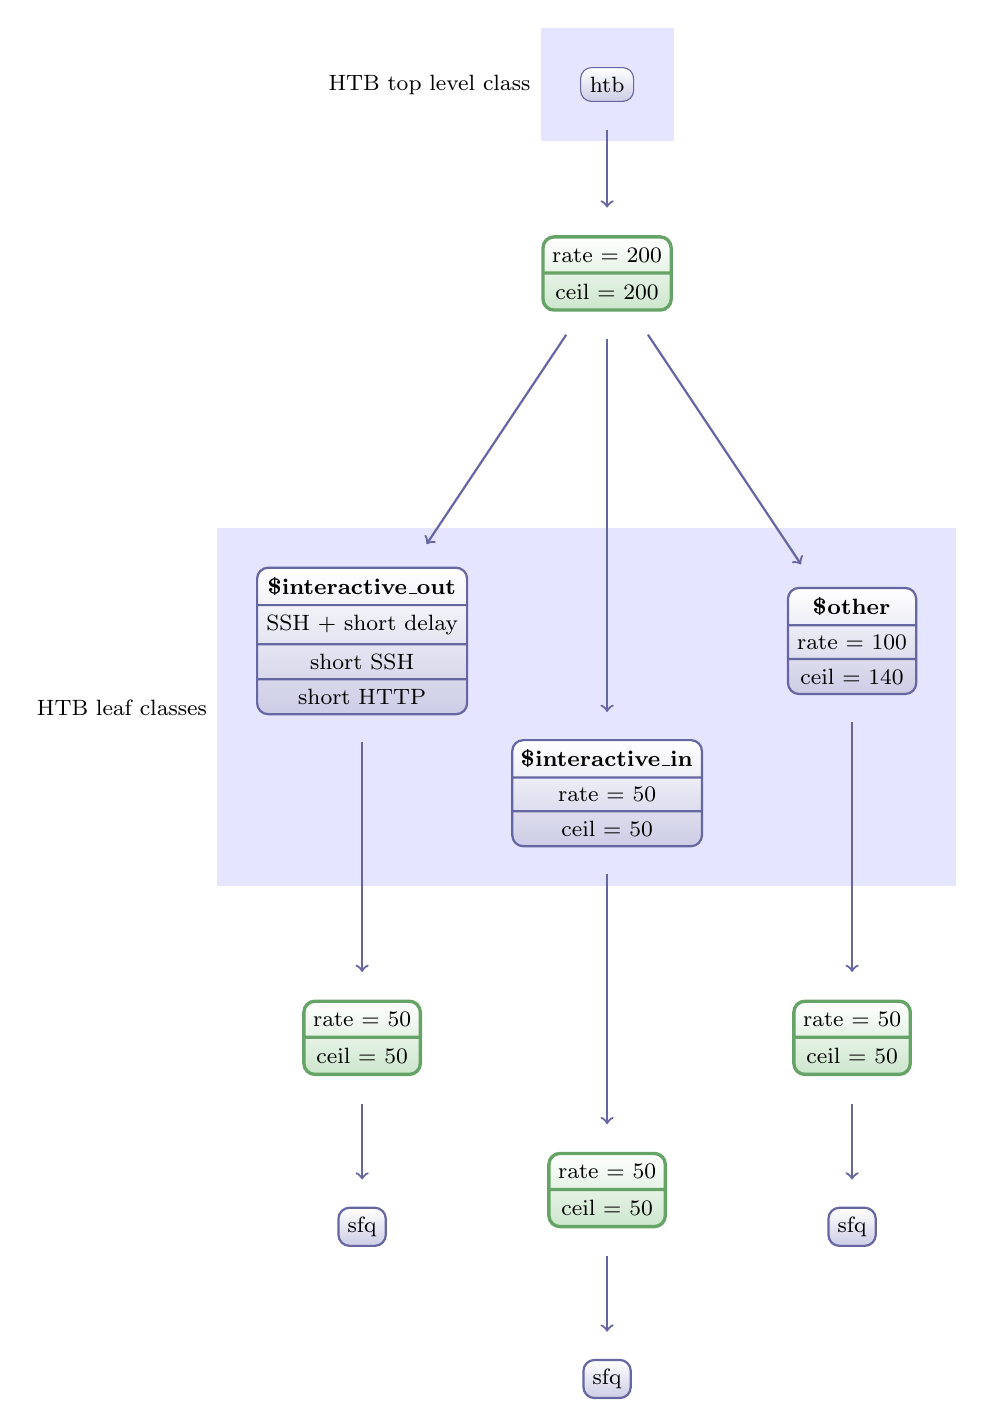
\begin{tikzpicture}[bend angle=45,auto,
    xscale						= 0.8,
	yscale						= 1.2,
	%every node/.style			= MyNodeStyle,
	grow						= south,
	%parent anchor				= west,
	%child anchor				= east,
    %sibling distance=3.5cm,level distance=2cm,
	%edge from parent/.style		= {black, ->, draw},
    punkt/.style={rectangle, rounded corners, shade, top color=white, bottom color=blue!50!black!20, draw=blue!40!black!60},
    %level 0/.style={level distance=2cm},
    level 1/.style={level distance=2cm},
    level 2/.style={sibling distance=10cm, level distance=5.5cm},
    level 3/.style={sibling distance=7cm,level distance=4.2cm},
    level 4/.style={sibling distance=2cm, level distance=2cm},
    %level 5/.style={sibling distance=1cm, level distance=2cm},
    descr/.style={rectangle split,rounded corners, shade, top color=white, bottom color=green!50!black!20, draw=green!40!black!60, very thick },
    %conn/.style={very thick,draw=blue!40!black!60,shorten >=10pt, shorten <=10pt, -> },
    pre/.style={thick, shorten >=10pt, shorten <=10pt, loosely dotted, <-},
    %FIXMEevery second punkt node part/.style={red},
    edge from parent/.style={draw=blue!40!black!60,shorten >=10pt, shorten <=10pt, -> ,thick},
    font=\footnotesize
    ]

\usetikzlibrary{trees,arrows,shapes,fit,backgrounds,topaths,positioning,fadings,decorations,automata}

\node[punkt] (root) {htb}
	%
    child {
        node [descr] [rectangle split parts=2, text ragged]% [label={left:beschränkung der Bandbreite}]
        (Interface)  (root-descr) {
            rate = 200%~{\kilo\bit\per\second}
            \nodepart{second} ceil = 200%~{\kilo\bit\per\second}
        }
        child [grow=south west] {
            node[punkt, rectangle split, rectangle split parts=4, text ragged] (interactive-out) {
                \textbf{\$interactive\_out}
                \nodepart{second} SSH + short delay
                \nodepart{third} short SSH
                \nodepart{fourth} short HTTP
            }
            child [grow=south] {
                node[descr, rectangle split, rectangle split parts=2, text ragged, level distance=6cm]% [label={left:beschränkung der Bandbreite}]
                (sfq-int-out-descr){
                rate = 50%~{\kilo\bit\per\second}
                \nodepart{second} ceil = 50%~{\kilo\bit\per\second}
                }
                child {
                    node[punkt]	(sfq-interactive-out) {sfq}
                }
            }
        }
        child [grow=south] {
            node[punkt, rectangle split, rectangle split parts=3, text ragged] (interactive-in) {
                \textbf{\$interactive\_in}
                \nodepart{second} rate = 50%~{\kilo\bit\per\second}
                \nodepart{third} ceil = 50%~{\kilo\bit\per\second}
            }
            child [grow=south] {
                node[descr, rectangle split, rectangle split parts=2, text ragged] (sfq-int-out-descr){
                rate = 50%~{\kilo\bit\per\second}
                \nodepart{second} ceil = 50%~{\kilo\bit\per\second}
                }
                child {
                    node[punkt] (sfq-interactive-in) {sfq}
                }
            }
        }
        child [grow=south east] {
            node[punkt, rectangle split, rectangle split parts=3, text ragged] (other) {
                \textbf{\$other}
                \nodepart{second} rate = 100%~{\kilo\bit\per\second}
                \nodepart{third} ceil = 140%~{\kilo\bit\per\second}
            }
            child [grow=south] {
                node[descr, rectangle split, rectangle split parts=2, text ragged] (sfq-int-out-descr){
                rate = 50%~{\kilo\bit\per\second}
                \nodepart{second} ceil = 50%~{\kilo\bit\per\second}
                }
                child {
                    node[punkt] (sfq-other) {sfq}
                }
            }
        }
    };
%\node [below of=sfq-interactive-in, rounded corners, shade, top color=white, bottom color=red!50!black!20, draw=red!40!black!60, below=2cm] (hardware) {Network-Interface}%
%                    edge [pre, bend left] (sfq-interactive-out)
%                    edge [pre] (sfq-interactive-in)
%                    edge [pre, bend right] (sfq-other);
%
\begin{pgfonlayer}{background}
  \node [fill=blue!10,fit=(root), inner sep=5mm,label={left:HTB top level class}] {};
  \node [fill=blue!10,fit=(interactive-out) (interactive-in) (other),inner sep=5mm,label={left:HTB leaf classes}] {};
  %\node [fill=blue!10,fit=(hardware),inner sep=5mm] {};
\end{pgfonlayer}

\end{tikzpicture}


